\section{Introduction}

When we ended the prequel with linear algebra, we found the complex number system to be highly useful in many ways.  We'll want to keep this in mind as we progress into further topics in the field of linear algebra.  Instead of dealing with transformations of finite dimensional vector spaces like $\R^n$ and $\C^n$, we will care about the spaces of functions on these spaces. So we find ourselves studying a bit of a nested structure.

Spaces of functions are of great importance.  In studying these spaces, we find ways to solve problems we will approach in the future (e.g., partial differential equations).  These spaces are, in some sense, infinite dimensional which means we can no longer draw pictures that accurately describe what is occuring.  Luckily enough, the intuition gained from the finite dimensional case will work just fine.  

We begin with complex functions as they are immensely fundamental in the study of the physical world and our mathematical development.  Once we have covered this area, we can adjust our view to the relevant spaces of functions that arise in areas such as quantum mechanics and partial differential equations in general.  As we did in the finite dimensional case, we can consider how these linear spaces transform under linear operators.  Finally, we make a nudge towards the spectral theory (eigenvalues and eigenvectors) via Fourier theory.

\section{Complex Functions}

In the prequel, we studied in depth single variable real valued functions $f\colon \R \to \R$. That is, functions with a single real variable as an input that outputs a single real number. Analogously, a \boldgreen{complex function} \index{complex function} is a function,  $f\colon \C \to \C$, with a complex number given as input and a complex number output as well.  The interesting quality to note is that we specified a complex number $z\in \C$ by putting
\[
z=x+iy,
\]
which means that single complex number is defined by two real numbers.  Recall as well that we could write a complex number in polar form
\[
z=re^{i\theta},
\]
which again requires the specification of two real numbers.  All of this is to say that we are allowed to (when it is helpful) think of complex functions as functions that input two real numbers $x,y\in \R$ and outputs two real numbers. Hence we would write $f\colon \R^2\to \R^2$.  The additional structure with complex numbers (in how we multiply them) forces us to think of $f\colon \C \to \C$ in a slightly different manner than their real valued counterparts which is why we cannot always make this identification!

\subsection{Cartesian and Polar Representations}

Consider a complex function $f\colon \C \to \C$.  Then, as always, we define this function by providing an output for each input and specify this by
\[
f(z)=w,
\]
where both $w\in \C$ and $z\in \C$ are complex numbers.  Hence, we can further decompose this function by writing
\[
f(z)=u(z)+iv(z),
\]
where $u(z)$ and $v(z)$ are real valued functions $u,v\colon \C \to \R$.  This decomposition is rather helpful in providing us a way to visualize the complex function $f$.  In this case, we are seeing what happens to the real $u(z)$ and imaginary part $v(z)$ of the output as we vary the complex input.

Of course, we can also write
\[
f(z)=r(z)e^{i\theta(z)},
\]
where again $r,\theta \colon \C \to \R$.  In this perspective, we are seeing what happens to the argument $\theta(z)$ and modulus $r(z)$ as we vary the complex input.  Which way of decomposing $f$ we choose is typically decided on the situation at hand.  It has more to do with the symmetry of the function than anything else! In this polar representation of the function, we refer to $\theta(z)$ as a \boldgreen{phase}.  



When we try to plot a complex function $f\colon \C \to \C$, we run into a bit of an issue.  When we plot real functions $g\colon \R\to \R$, we can draw this in a 2-dimensional plane. However, if we were to draw a complex function using the same idea, it would be in a 4-dimensional space. This cannot work.  But that doesn't mean we are out of options!

Remember, we can think of a point $z$ in the complex plane as a 2-dimensional vector. So, for example, if we take $z_1=1+i$ and $z_2 = 1-2i$, we can plot this like
\[
        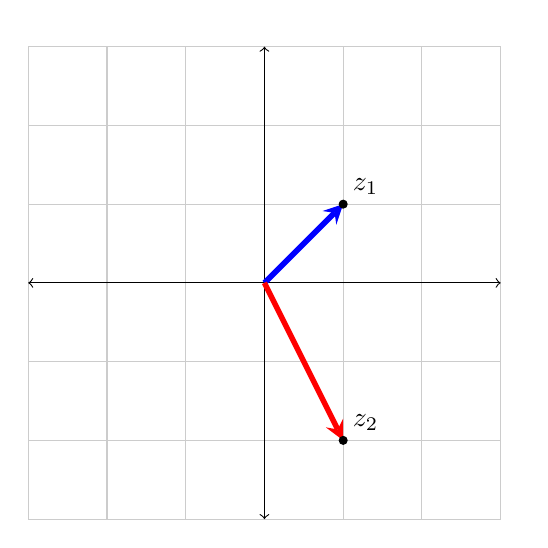
\begin{tikzpicture}
        \draw[thin,gray!40] (-3,-3) grid (3,3);
        \draw[<->] (-3,0)--(3,0) node[right]{$\RE$};
        \draw[<->] (0,-3)--(0,3) node[above]{$\IM$};
        \draw[line width=2pt,blue,-stealth](0,0)--(1,1) node[anchor=east] at (1,1){};
        \draw[line width=2pt,red,-stealth](0,0)--(1,-2) node[anchor=east] at (1,-2){};
        \foreach \Point/\PointLabel in {(1,1)/z_1, (1,-2)/z_2}
        \draw[fill=black] \Point circle (0.05) node[above right] {$\PointLabel$};
        \end{tikzpicture}
\]
Using this idea, let us see how we can plot a complex function in a different way.

\begin{ex}{Plotting a Complex Function}{plot_complex_func}
	Let's consider a complex function $f\colon \C \to \C$ given by the function
	\[
		f(z) = iz= -\IM(z)+i\RE(z).
	\]
	Recall that multiplication by $i$ rotates a complex number by an angle of $\pi/2$ in the counterclockwise direction. Thinking this way will help us understand what this function is doing.  For some more concrete results, we should compute a few values for this function
	\begin{align*}
		f(0)&= 0 & f(1)&=i & f(i)&= -1\\
		f(-1)&= -i & f(1+i)&= -1+i & f(-1 -i) &= 1 - i.
	\end{align*}
	We can plot these values as vectors emanating from the input point $z$. That is, we can place the arrow given by the output $f(z)$ at the point $z$.  
	\[
	        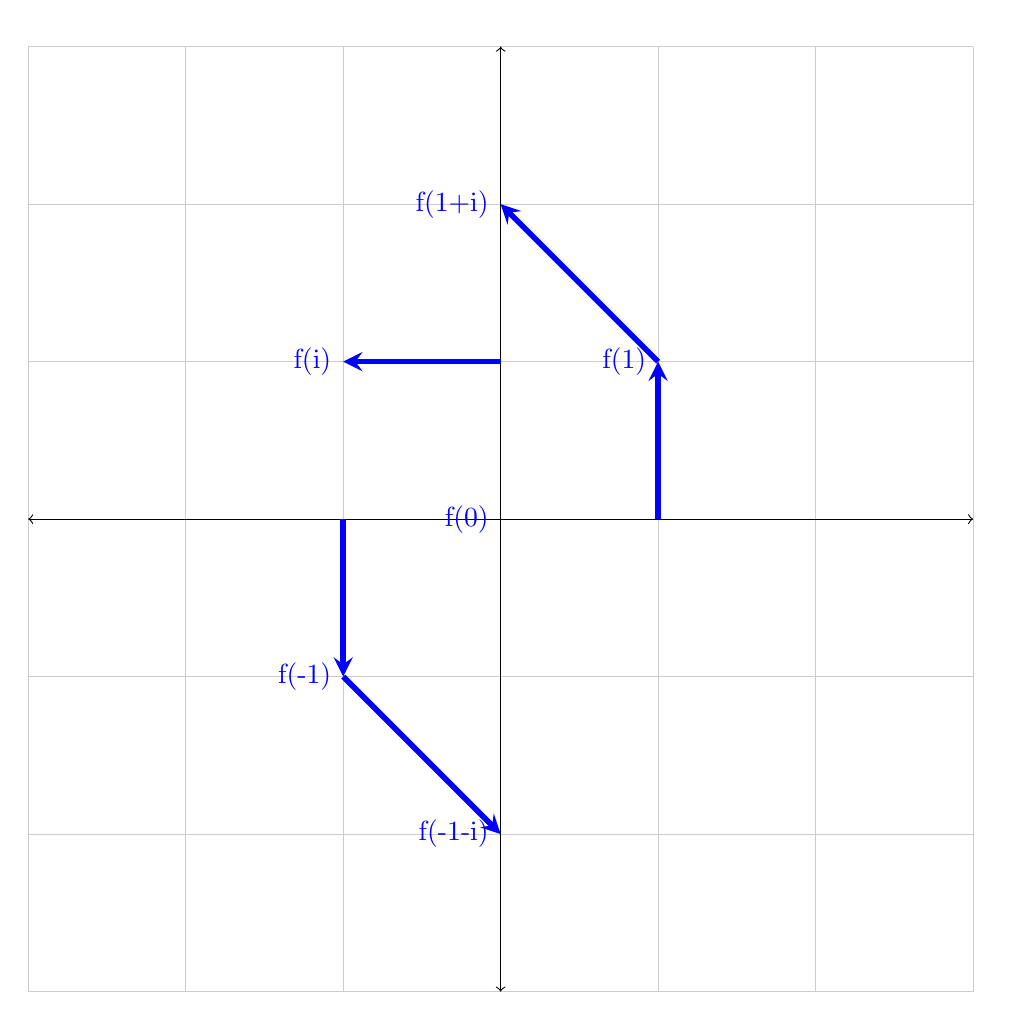
\begin{tikzpicture}[scale=2]
	        \draw[thin,gray!40] (-3,-3) grid (3,3);
	        \draw[<->] (-3,0)--(3,0) node[right]{$\RE$};
	        \draw[<->] (0,-3)--(0,3) node[above]{$\IM$};
	        \draw[line width=2pt,blue,-](0,0)--(0,0) node[anchor=east] at (0,0){f(0)};
	        \draw[line width=2pt,blue,-stealth](1,0)--(1,1) node[anchor=east] at (1,1){f(1)};
	        \draw[line width=2pt,blue,-stealth](-1,0)--(-1,-1) node[anchor=east] at (-1,-1){f(-1)};
	        \draw[line width=2pt,blue,-stealth](0,1)--(-1,1) node[anchor=east] at (-1,1){f(i)};
	        \draw[line width=2pt,blue,-stealth](1,1)--(0,2) node[anchor=east] at (0,2){f(1+i)};
	        \draw[line width=2pt,blue,-stealth](-1,-1)--(0,-2) node[anchor=east] at (0,-2){f(-1-i)};
	        \end{tikzpicture}
	  \]
	  We can then do this for many more input points to get a picture like the following.
		\begin{figure}[H]
			\centering
			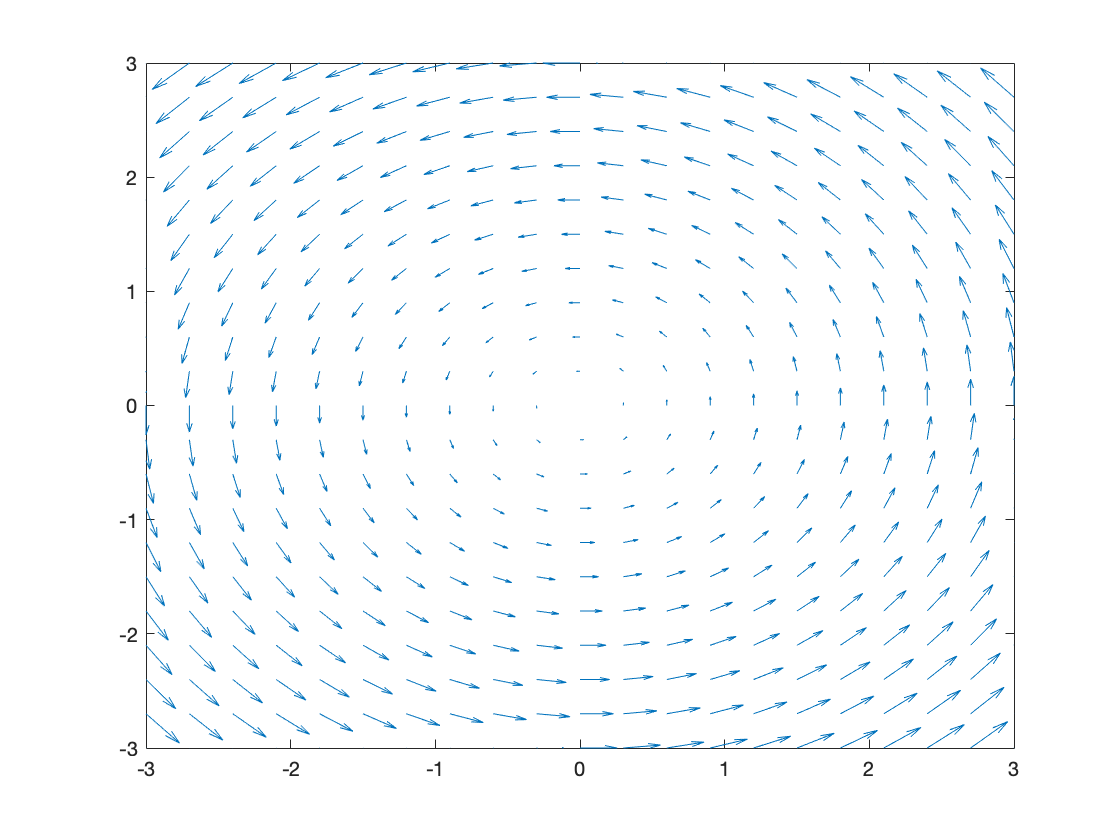
\includegraphics[width=\textwidth]{Figures_Part_5/complex_function_visual.png}
			\caption{A plot of various different outputs for their corresponding inputs.}
		\end{figure}
		What we see here is typically referred to as a vector field. We will get to this notion later on in the text.
\end{ex}
		
\subsection{Complex Valued Functions}

A major focus in this course is understanding the mathematics behind quantum mechanics.  For a chemist, this knowledge is rather important since modern theory is mostly quantum in nature.  What isn't quantum is likely thermodynamical or electrodynamical in nature and we will get to these topics a bit later on. 

Recall that wavefunctions are solutions to Schr\"odinger's equation.  In the broadest generality, wavefunctions are functions that are complex valued and whose domain of definition is on some region $\Omega$ in space $\R^3$.  More generally, we can allow for $\Omega$ to a be a region in other spaces as well. To restate this, we are considering a function of the form $\Psi\colon \Omega \to \C$ where we will specify what the domain $\Omega$ is. Previously, we looked at models in lower dimensions (e.g., the free particle in the 1-dimensional box) since we have yet to properly discuss multivariate functions.  

For now, consider a complex function $\Psi\colon [a,b] \to \C$ that has a single real variable as an input.  Thus, we define this function by $\Psi(x)=z$, where $z\in \C$.  Of course, we get the Cartesian decomposition
\[
\Psi(x)=u(x)+iv(x),
\]
or the polar decomposition
\[
\Psi(x)=r(x)e^{i\theta(x)}.
\]

The great thing in this case is that we can differentiate and integrate wavefunctions in a way that's no different than single variable real functions!  Fundamentally, this is due to the fact that our understanding of the derivative has only been defined for a single real value input. We will deepen our understanding later.  So, for a wavefunction we have that
\[
\Psi'(x)=u'(x)+iv'(x),
\]
and in the polar case we have
\[
\Psi'(x)=r'(x)e^{i\theta(x)}+r(x)e^{i\theta(x)}\theta'(x),
\]
which follows from the chain rule.

\begin{exercise}
	Verify the polar derivative above is correct.
\end{exercise}

Integration follows the fundamental theorem of calculus and hence we have
\[
\int_a^b \Psi'(x)dx = \Psi(b)-\Psi(a).
\]
So, for example, in the cartesian representation we have
\[
\int_a^b \Psi'(x)dx = \int_a^b u'(x)dx+i\int_a^b v'(x)dx = [u(b)-u(a)]+i[v(b)-v(a)].
\]

\begin{remark}
	Complex functions (i.e., functions with complex valued inputs) have different behavior with integration and differentiation which we will not discuss at all.  The closest we will get to this structure is calculus in $\R^2$.
\end{remark}

\begin{ex}{A Line in $\C$}{line_in_C}
	Let's consider the complex function $f\colon \R \to \C$ given by the Cartesian representation 
	\[
	f(x) = x+ix.
	\]
	How should we think of this function? For one, we can see how the output changes as the input changes by testing a few values
	\begin{align*}
		f(0)&=0 & f(1)&=1+i\\
		f(-1)&=-1-i & f(2)&=2+2i.
	\end{align*}
	We can also visualize this function in the following way. For every input, we will just place the complex output into the complex plane. Unlike plotting real functions, we will have to pay a bit more attention to what the input value is.
	\[
	    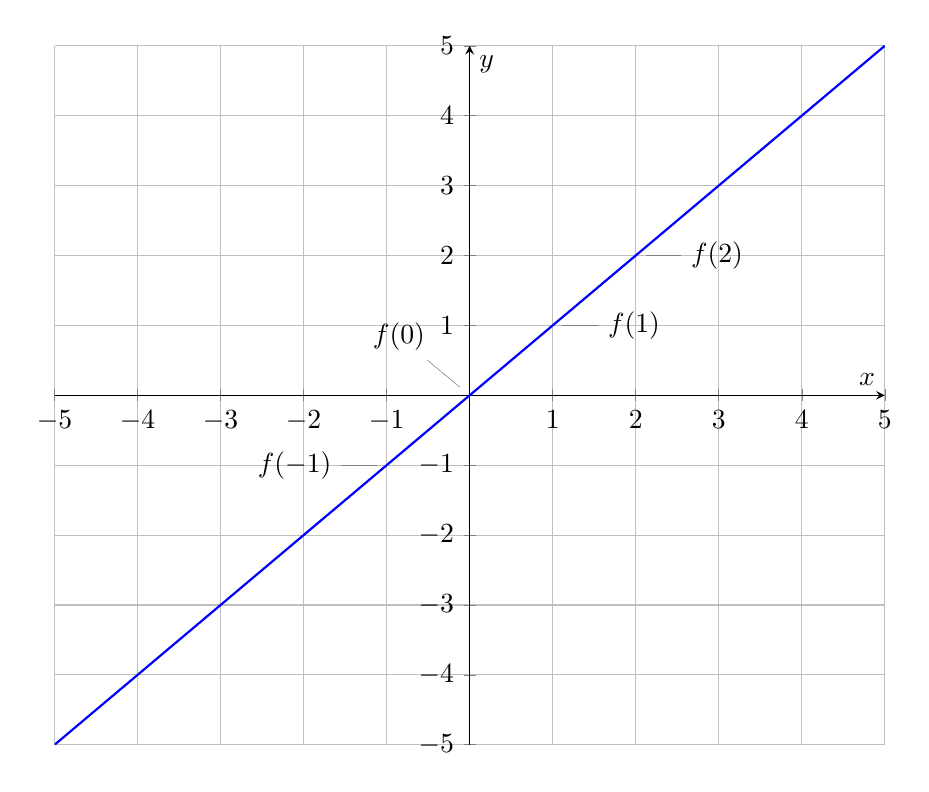
\begin{tikzpicture}[baseline]
	    \begin{axis}[
	    axis y line=center,
	    axis x line=middle,
	    %axis equal,
	    grid=both,
	    xmax=5,xmin=-5,
	    ymin=-5,ymax=5,
	    xlabel=$x$,ylabel=$y$,
	    xtick={-10,...,10},
	    ytick={-10,...,10},
	    width=\textwidth,
	    anchor=center,
	    ]
	    \addplot [mark=none, blue, thick]{x} ;
	    \addplot [mark=none] coordinates {(1,1)} node[pin=0:{$f(1)$}]{};
	    \addplot [mark=none] coordinates {(2,2)} node[pin=0:{$f(2)$}]{};
	    \addplot [mark=none] coordinates {(-1,-1)} node[pin=180:{$f(-1)$}]{};
	    \addplot [mark=none] coordinates {(0,0)} node[pin=135:{$f(0)$}]{};
	    \end{axis}
	    \end{tikzpicture}
	    \]
	   We often refer to this type of function as a curve or, in the complex case specifically, a contour.  Again, we will revisit curves later on in this text.
\end{ex}

\begin{ex}{Wavefunctions in the Box}{wavefunctions_in_1dbox}
	Let $\Omega=[0,L]$ and recall that the normalized states of the particle in the 1-dimensional box were given by
	\[
		\psi_n(x)=\sqrt{\frac{2}{L}} \sin\left(\frac{n \pi x}{L}\right).
	\]
	Recall as well that we could write a wavefunction as a superposition of states by
	\[
		\Psi(x)=\sum_{n=0}^\infty a_n \psi_n(x).
	\]
	Though these states are real valued, there is no physics that requires this.  Similarly, the coefficients $a_n$ are also not constrained to be real valued constants either.  In the broadest generality, $\Psi$ can be a complex valued function and the coefficients $a_n$ can be complex as well.

	Fundamentally, this is due to the physical understanding of the solutions to Schr\"odinger's equation. When we are looking for physically meaningful interpretations of a wavefunction, we must evaluate an integral. We can think of this act of integration as performing a measurement.  For example, let $[a,b]$ be a subinterval of $[0,L]$, then we can compute the probability of the particle with wavefunction $\Psi(x)$ to be in the region $[a,b]$ by 
	\[
		P_{[a,b]}(\Psi) = \int_a^b \|\Psi(x)\|^2dx,
	\]
	where we have the pointwise modulus of the complex valued function
	\[
		\|\Psi(x)\|^2 = \Psi^*(x)\Psi(x),
	\]
	where $~^*$ indicates the complex conjugate.  Say we take the cartesian representation for $\Psi(x)$ by $\Psi(x)=u(x)+iv(x)$, then
	\[
		\|\Psi(x)\|^2 = u^2(x)+v^2(x).
	\]
	
	Let $\Psi(x)=\frac{1}{\sqrt{2}}\psi_1(x)+\frac{1}{\sqrt{2}}\psi_2(x)$ be a superposition state.  We can compute the probability that the particle is in the first half of the region $[0,L]$ by computing
	\begin{align*}
		P_{[0,L/2]}(\Psi)&=\int_{0}^{L/2}  \|\Psi(x)\|^2 dx \\
			&=\int_{0}^{L/2} \frac{1}{2}\psi_1^2(x)+ \psi_1(x)\psi_2(x)+\frac{1}{2}\psi_2^2(x)dx\\
			&=\int_{0}^{L/2}\frac{1}{2} \left(\sqrt{\frac{2}{L}}\sin\left(\frac{\pi x}{L}\right)\right)^2 + \sqrt{\frac{2}{L}}\sin\left(\frac{\pi x}{L}\right)\sin\left(\frac{2\pi x}{L}\right)+ \frac{1}{2}\left(\sqrt{\frac{2}{L}}\sin\left(\frac{2\pi x}{L}\right)\right)^2dx\\
			&=\frac{1}{2}+\frac{4}{3\pi}\\
			&\approx .924.
	\end{align*}
	Through this calculation we have found that the probability that the particle is the first half of box is about $92.5\%$.  Since the particle must be in the box, it follows that the probability of the particle being in $[L/2,L]$ must be $1-\frac{1}{2}-\frac{4}{3\pi}$ or roughly $7.5\%$.  This is quite different than we would expect classically!

	We can plot the functions used above to see why this is the case.
	\begin{figure}[H]
	\centering
		\begin{subfigure}[h]{0.49\textwidth}
			\centering
			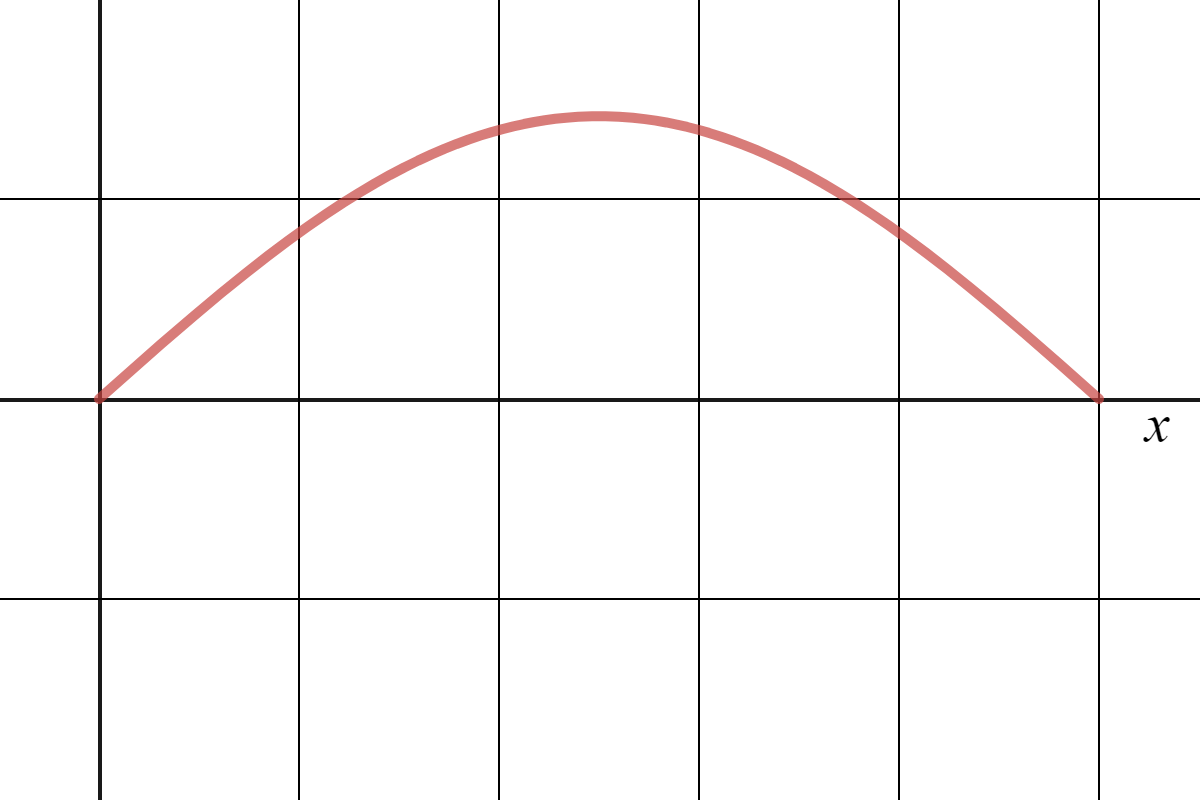
\includegraphics[width=.8\textwidth]{Figures_Part_5/psi_1.png}
			\caption{Normalized state $\psi_1(x)$.}
		\end{subfigure}
		~
		\begin{subfigure}[h]{0.49\textwidth}
			\centering
			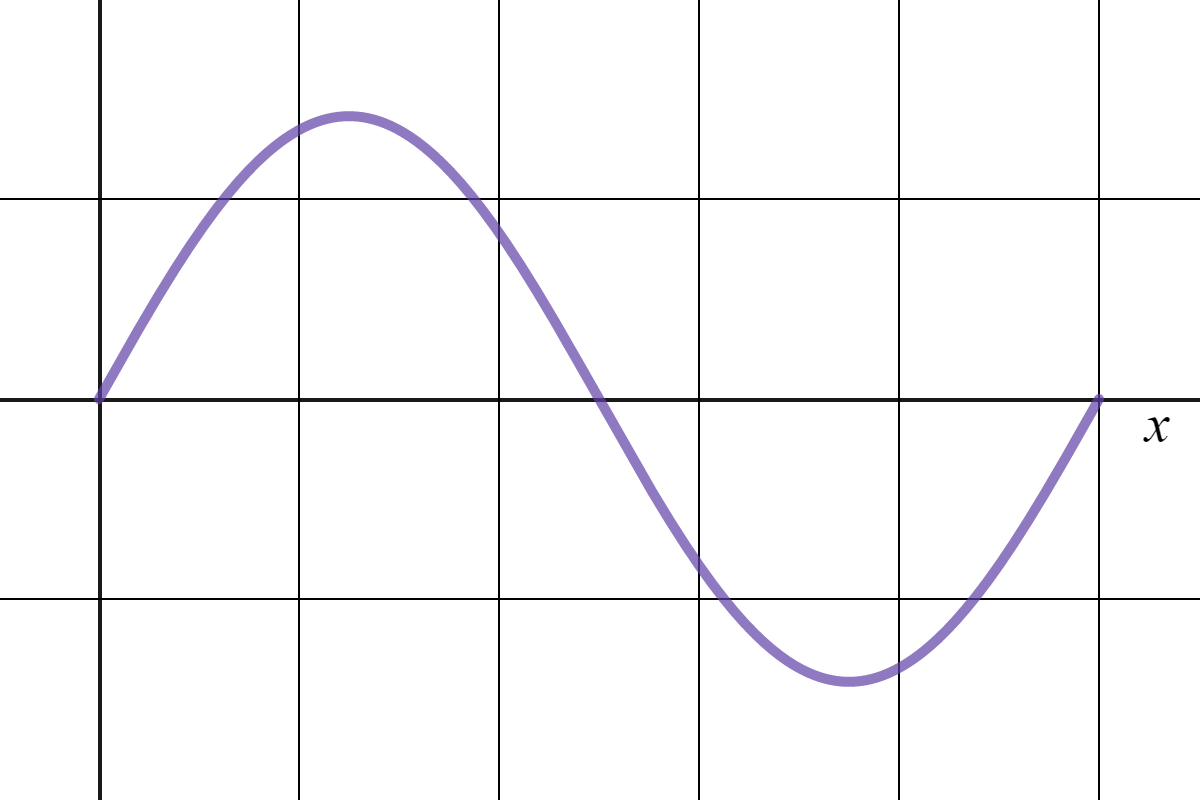
\includegraphics[width=.8\textwidth]{Figures_Part_5/psi_2.png}
			\caption{Normalized state $\psi_2(x)$.}
		\end{subfigure}
		\\
		\begin{subfigure}[h]{0.49\textwidth}
			\centering
			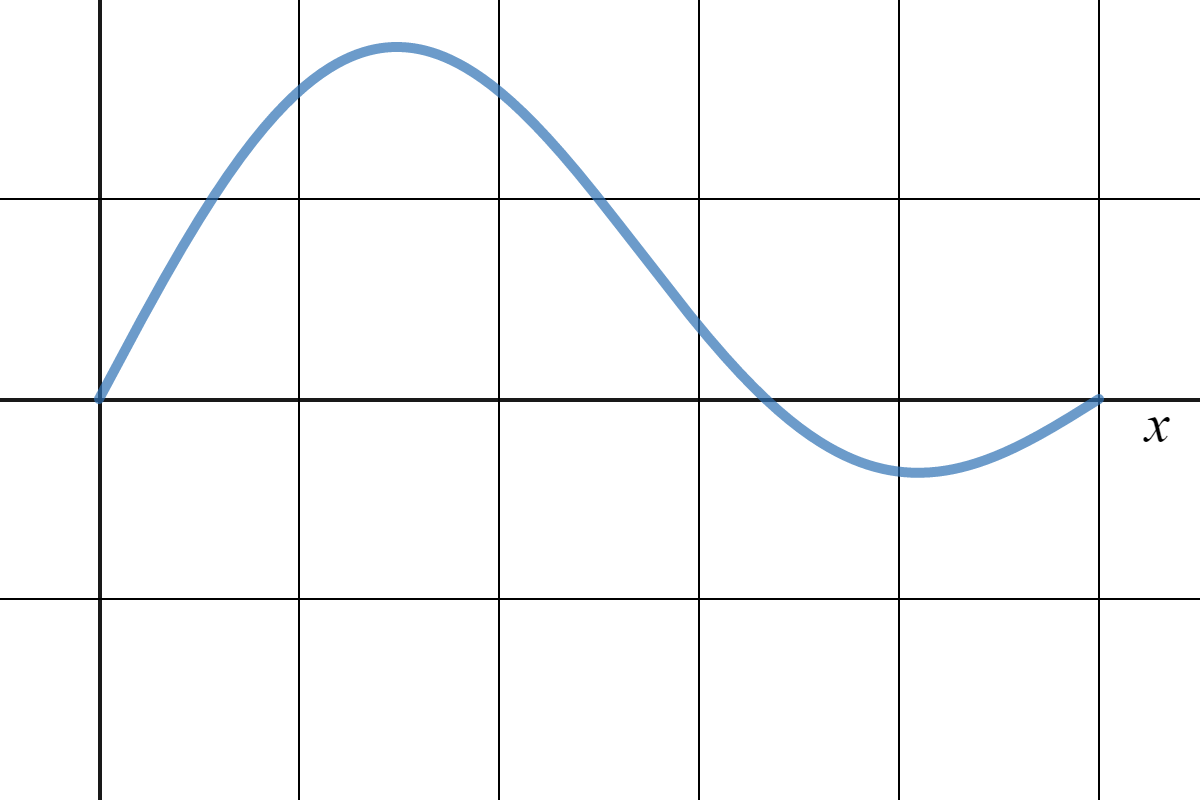
\includegraphics[width=.8\textwidth]{Figures_Part_5/Psi.png}
			\caption{The wavefunction $\Psi(x)$.}
		\end{subfigure}
		~
		\begin{subfigure}[h]{0.49\textwidth}
			\centering
			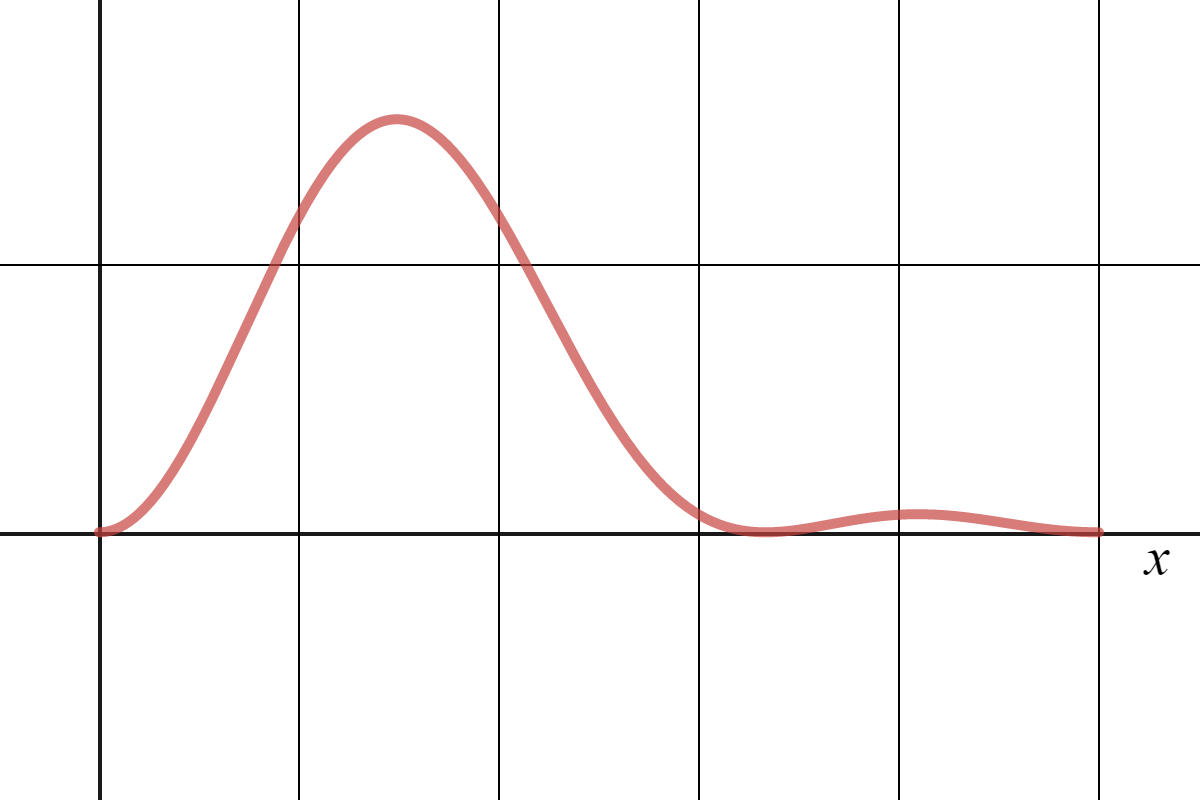
\includegraphics[width=.8\textwidth]{Figures_Part_5/prob_Psi.png}
			\caption{The probability function $\|\Psi(x)\|^2$.}
		\end{subfigure}
	\end{figure}
	The plots above of course show us that the integration makes sense.  We can see in (d) that the function that describes the probability is heavily weighted towards the first half of the interval $[0,L]$. One may then wonder if this is always true? That is, if I were to check back later in time, is the probability still distributed in the same way? The answer is no.  Later, we will introduce the time dependent version of the Schr\"odinger equation where we will see that these wavefunctions also evolve over time.  To some extent, we can see a bit of this behavior now.
	
	If we instead change our wavefunction by introducing a phase difference for each of the components.  What will happen in this case? If you have seen the double slit experiment, you may guess that introducing a phase difference can change the result (as phase difference causes interference). Instead of the $\Psi(x)$ above, take 
	\[
		\tilde{\Psi}(x) = \frac{e^{i\theta}}{\sqrt{2}} \psi_1(x) + \frac{e^{i\phi}}{\sqrt{2}} \psi_2(x).
	\]
	In this case, all we have done is made the wavefunction complex.  If, however, we consider the probability distribution given by this new wave function, we find
	\[
		\|\tilde{\Psi}(x)\|^2 = \tilde{\Psi}^*(x)\tilde{\Psi}(x) = \frac{1}{2}\psi_1^2(x)+\frac{e^{i(\theta-\phi)}}{2}\psi_1(x)\psi_2(x)+\frac{e^{i(\phi-\theta)}}{2}\psi_1(x)\psi_2(x)+\frac{1}{2}\psi_2^2(x).
	\]
	This is now slightly different! However, we can note that
	\[
		\frac{e^{i(\theta-\phi)}+e^{i(\phi-\theta)}}{2} = \cos(\theta-\phi),
	\]
	and hence we have
	\[
		\|\tilde{\Psi}(x)\|^2 = \tilde{\Psi}^*(x)\tilde{\Psi}(x) = \frac{1}{2}\psi_1^2(x)+\cos(\theta-\phi)\psi_1(x)\psi_2(x)+\frac{1}{2}\psi_2^2(x).
	\]
	So the phase difference $\delta=|\theta-\phi|$ between the two states causes the wavefunction to change. In the first example with $\Psi(x)$, the phase difference $\delta=0$ and we observed the probability function $\|\Psi(x)\|^2$.  However, let us see what happens as we change the phase.
	\begin{figure}[H]
	\centering
		\begin{subfigure}[h]{0.49\textwidth}
			\centering
			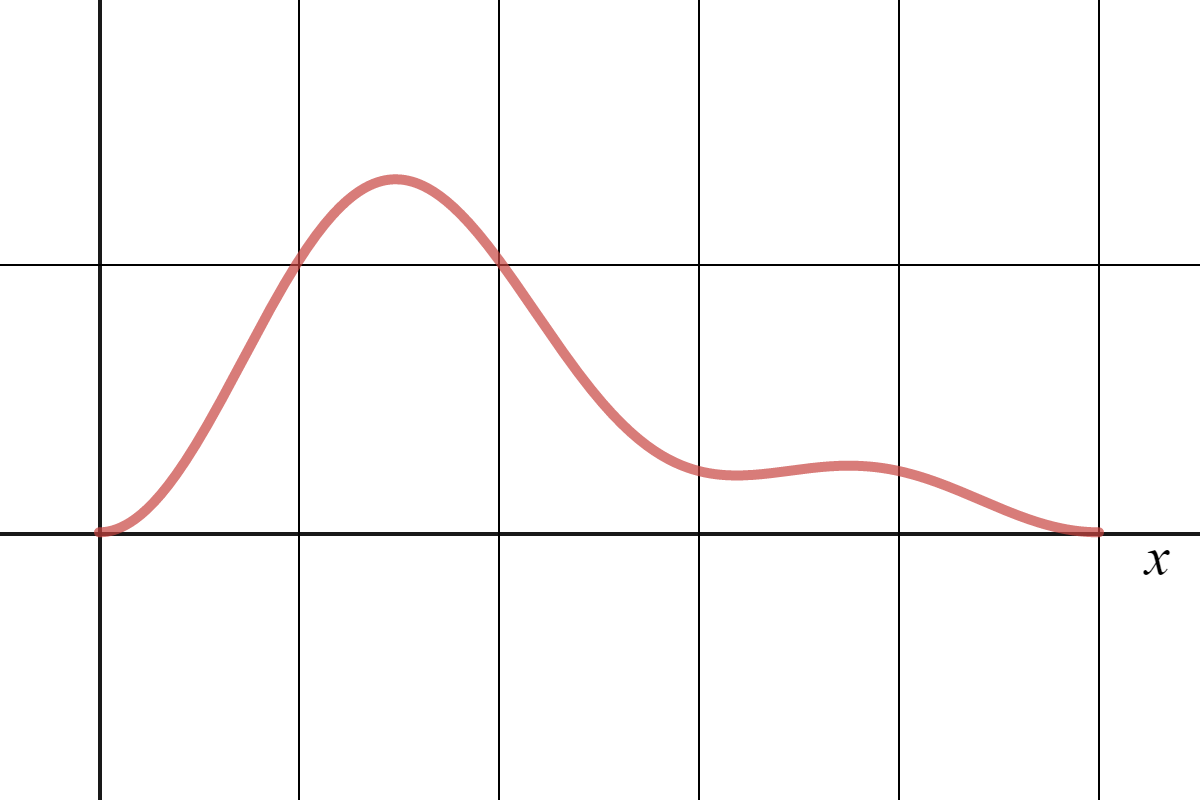
\includegraphics[width=.8\textwidth]{Figures_Part_5/prob_Psi_pi4.png}
			\caption{Phase difference $\delta=0$.}
		\end{subfigure}
		~
		\begin{subfigure}[h]{0.49\textwidth}
			\centering
			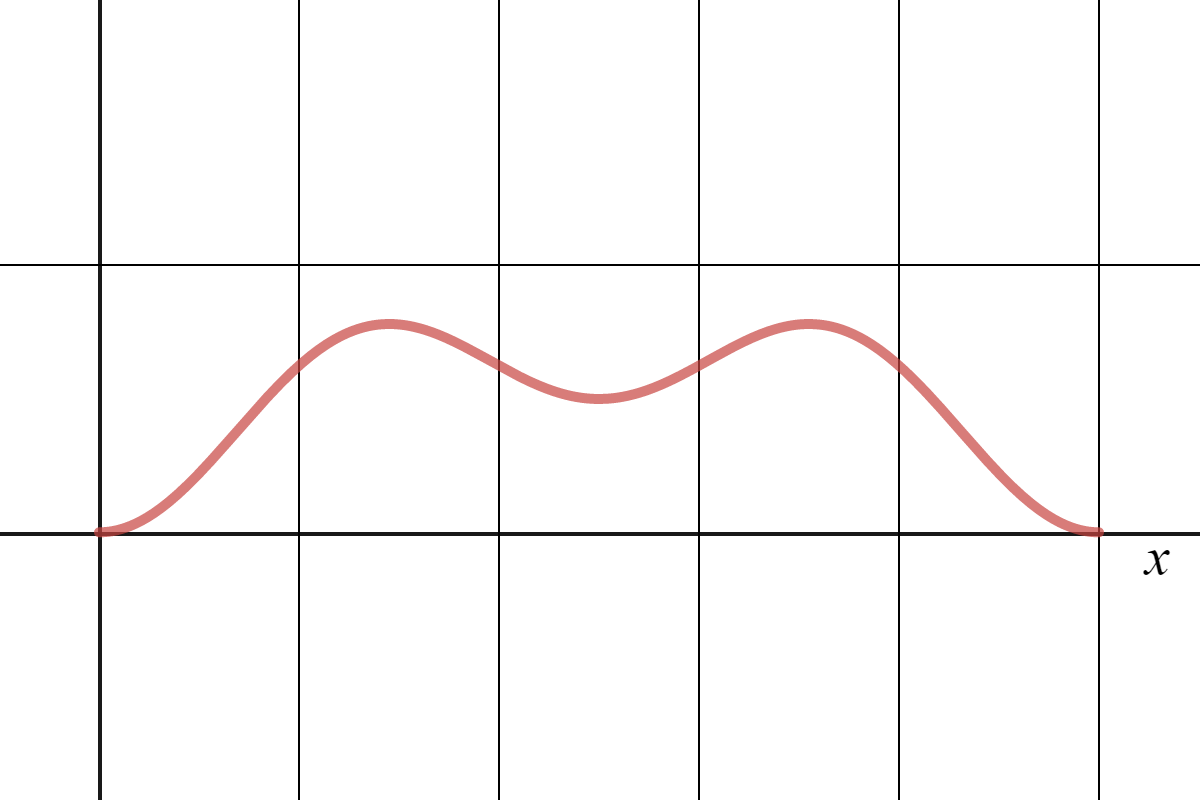
\includegraphics[width=.8\textwidth]{Figures_Part_5/prob_Psi_pi2.png}
			\caption{Phase difference $\delta=\frac{\pi}{3}$.}
		\end{subfigure}
		\\
		\begin{subfigure}[h]{0.49\textwidth}
			\centering
			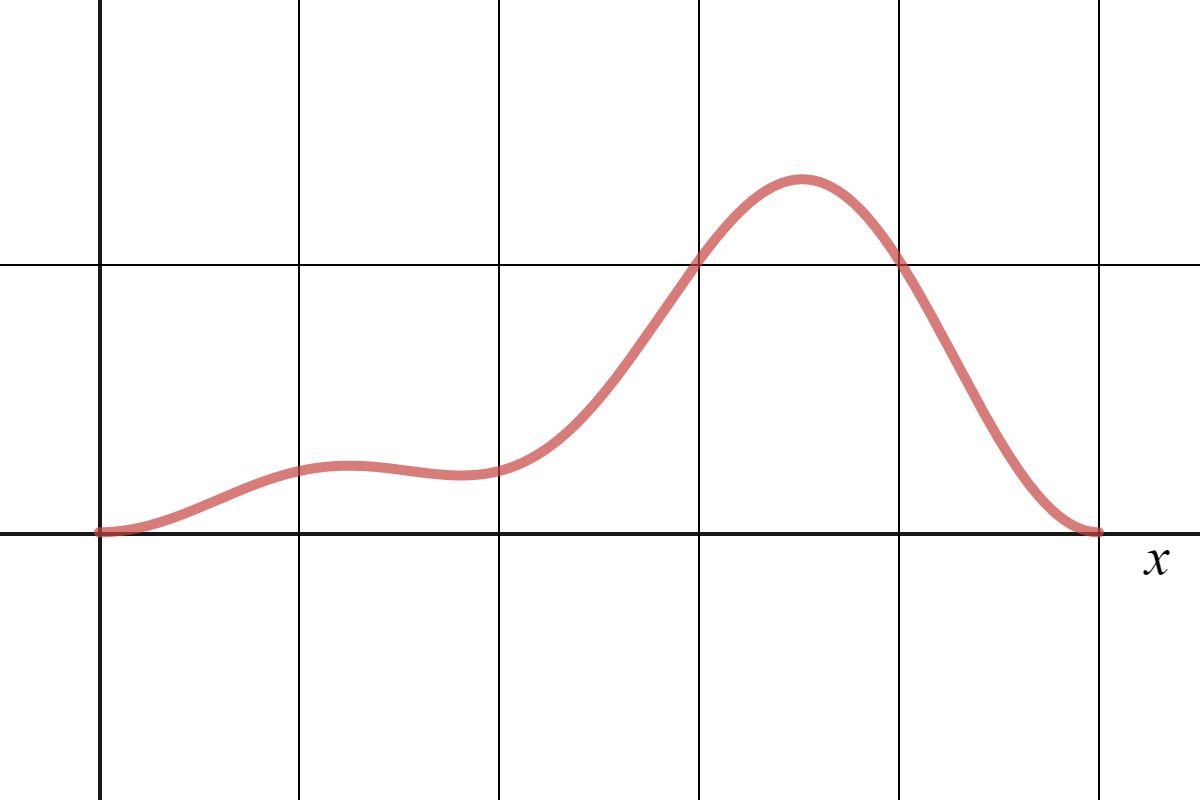
\includegraphics[width=.8\textwidth]{Figures_Part_5/prob_Psi_3pi4.png}
			\caption{Phase difference $\delta=\frac{2\pi}{3}$.}
		\end{subfigure}
		~
		\begin{subfigure}[h]{0.49\textwidth}
			\centering
			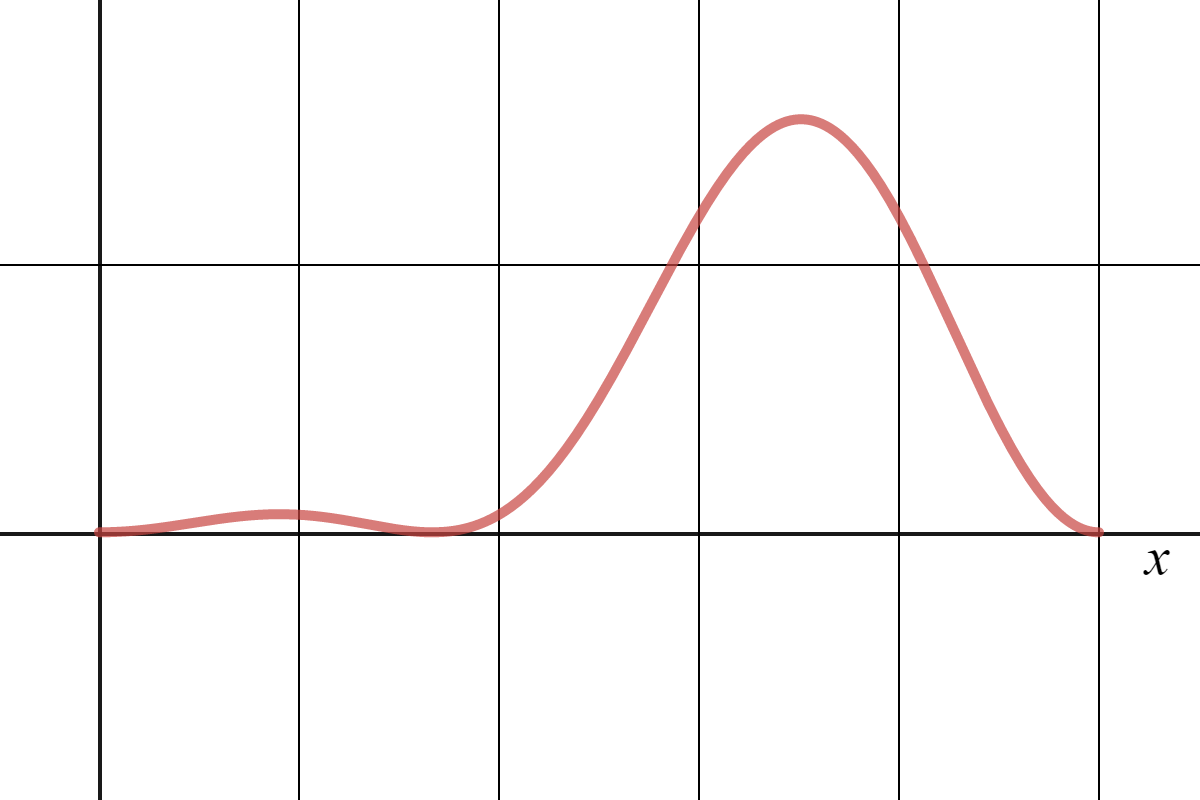
\includegraphics[width=.8\textwidth]{Figures_Part_5/prob_Psi_pi.png}
			\caption{Phase difference $\delta=\pi$.}
		\end{subfigure}
	\end{figure}
	 Interestingly enough, it seems that the phase difference ``moves" the particle around in the box. Of course, the particle itself is not moving, but the function that represents the likelihood of its position changes as the phase changes.  The largest difference in phase is $\pi$, and when we see this, we find that the distribution given by $\|\tilde{\Psi}(x)\|^2$ is the mirror image of the original $\|\Psi(x)\|^2$.  

	There are two important remarks to note here.
	\begin{enumerate}[1.]
		\item We can change the global phase of the system without changing the probability of measurement.  That is, $e^{i\theta}\Psi(x)$ has no discernable difference from $\Psi(x)$ (you can verify this from the work above).
		\item This difference in phase seems to drive some form of motion for a particle.  It is with this insight that we will later revisit the time dependent version of the Schr\"odinger equation and see how the time component relates to phase.
	\end{enumerate}
\end{ex}

\begin{remark}
	In a sense, the integral defined above $P_{[a,b]}(\Psi)$ is a real valued function with a function as an input.  Though we have not noted this until now, it becomes important in the future.
\end{remark}

All of this is to say that we must be able to work with complex valued functions.  They show up in physics and help us describe what we observe through nature.  It's important to remember that all measurements we make in a lab must be real valued, and so our mathematical models for these measurements must take that into account as well.